\documentclass[aspectratio=169,10pt,t,german,xcolor=table]{beamer}
\usepackage{../../common/beamer-cgs-lecture}

\title{Gem Illuminator}
\author{Pascal Lange, Sebastian Koall, Jennifer Stamm}
\institute{\translate{Hasso Plattner Institute}}
\date{WiSe~2014/2015}

\subtitle{Game Programming}
\titlegraphic{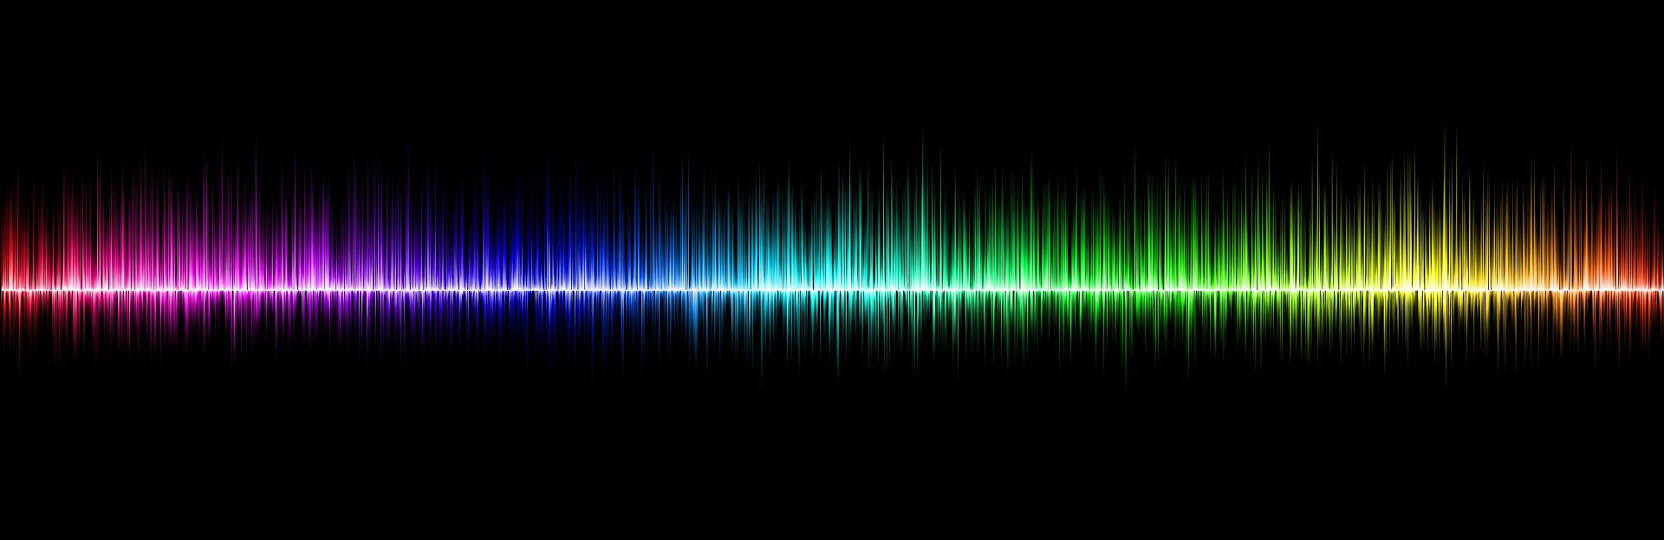
\includegraphics[width=\linewidth]{images/teaser}}

\begin{document}

% < 1m
\slidetitle
\section*{Abschlusspräsentation}

% 1m
\slideonetoonegraphics
{Motivation und Spielidee}
{images/start-situation}
{}
{images/lichteffekt-diffus-reflektion}
{}



% 3m
\begin{frame}{Demo}
	%TODO Aktueller Screenshot/Video
	\centering
	\includemedia[
	width=0.8\textwidth,height=0.8\textheight,
	activate=pageopen,
	flashvars={
		modestbranding=1 % no YT logo in control bar
		&autohide=1 % controlbar autohide
		&showinfo=0 % no title and other info before start
		&rel=0 % no related videos after end
	},
	url % Flash loaded from URL
	]{}{http://www.youtube.com/v/pz10FPVzF1k}
\end{frame}

% 1m
\begin{frame}{Architektur -- Zwischenstandspräsentation}
	\begin{figure}
		\centering
		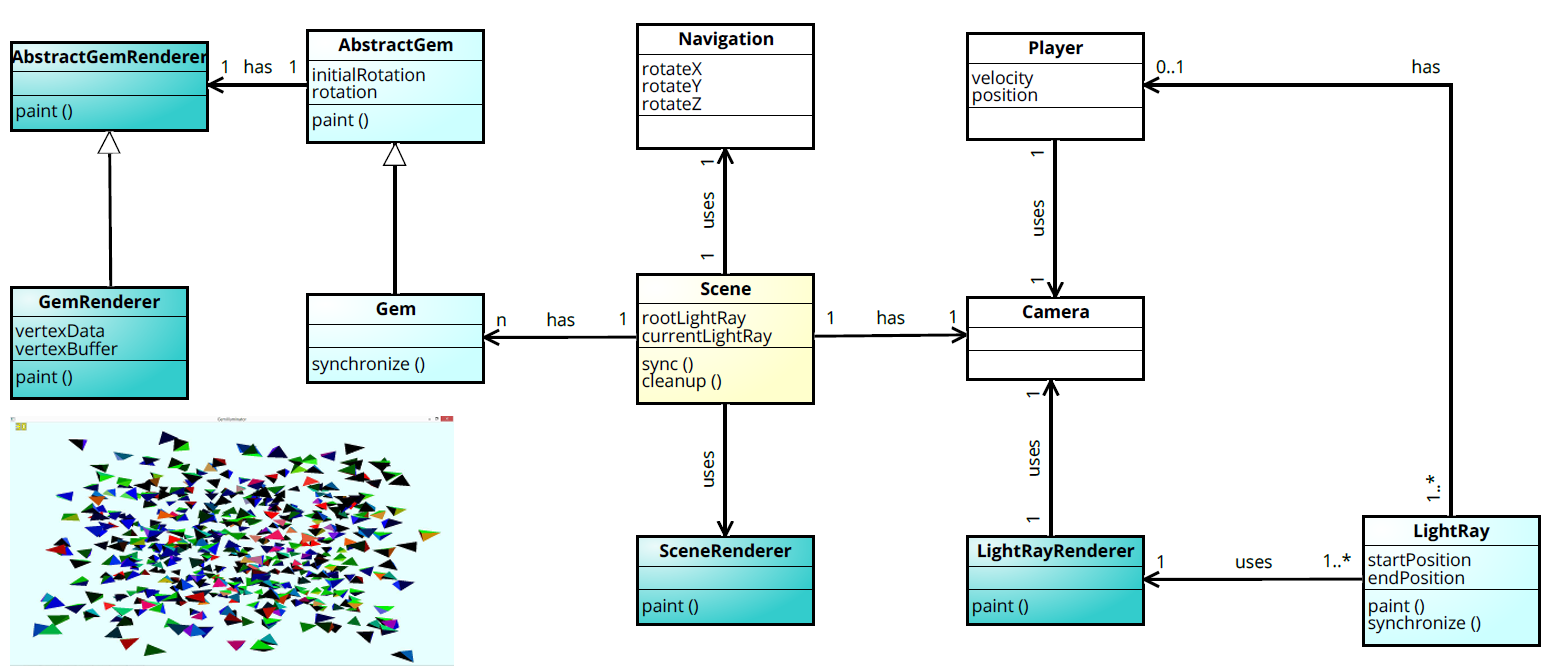
\includegraphics[width=\textwidth, height=0.7\textheight, keepaspectratio]{images/klassendiagramm}
	\end{figure}
\end{frame}

% 4m
\begin{frame}{Architektur -- Abschlusspräsentation}
	\begin{figure}
		\centering
		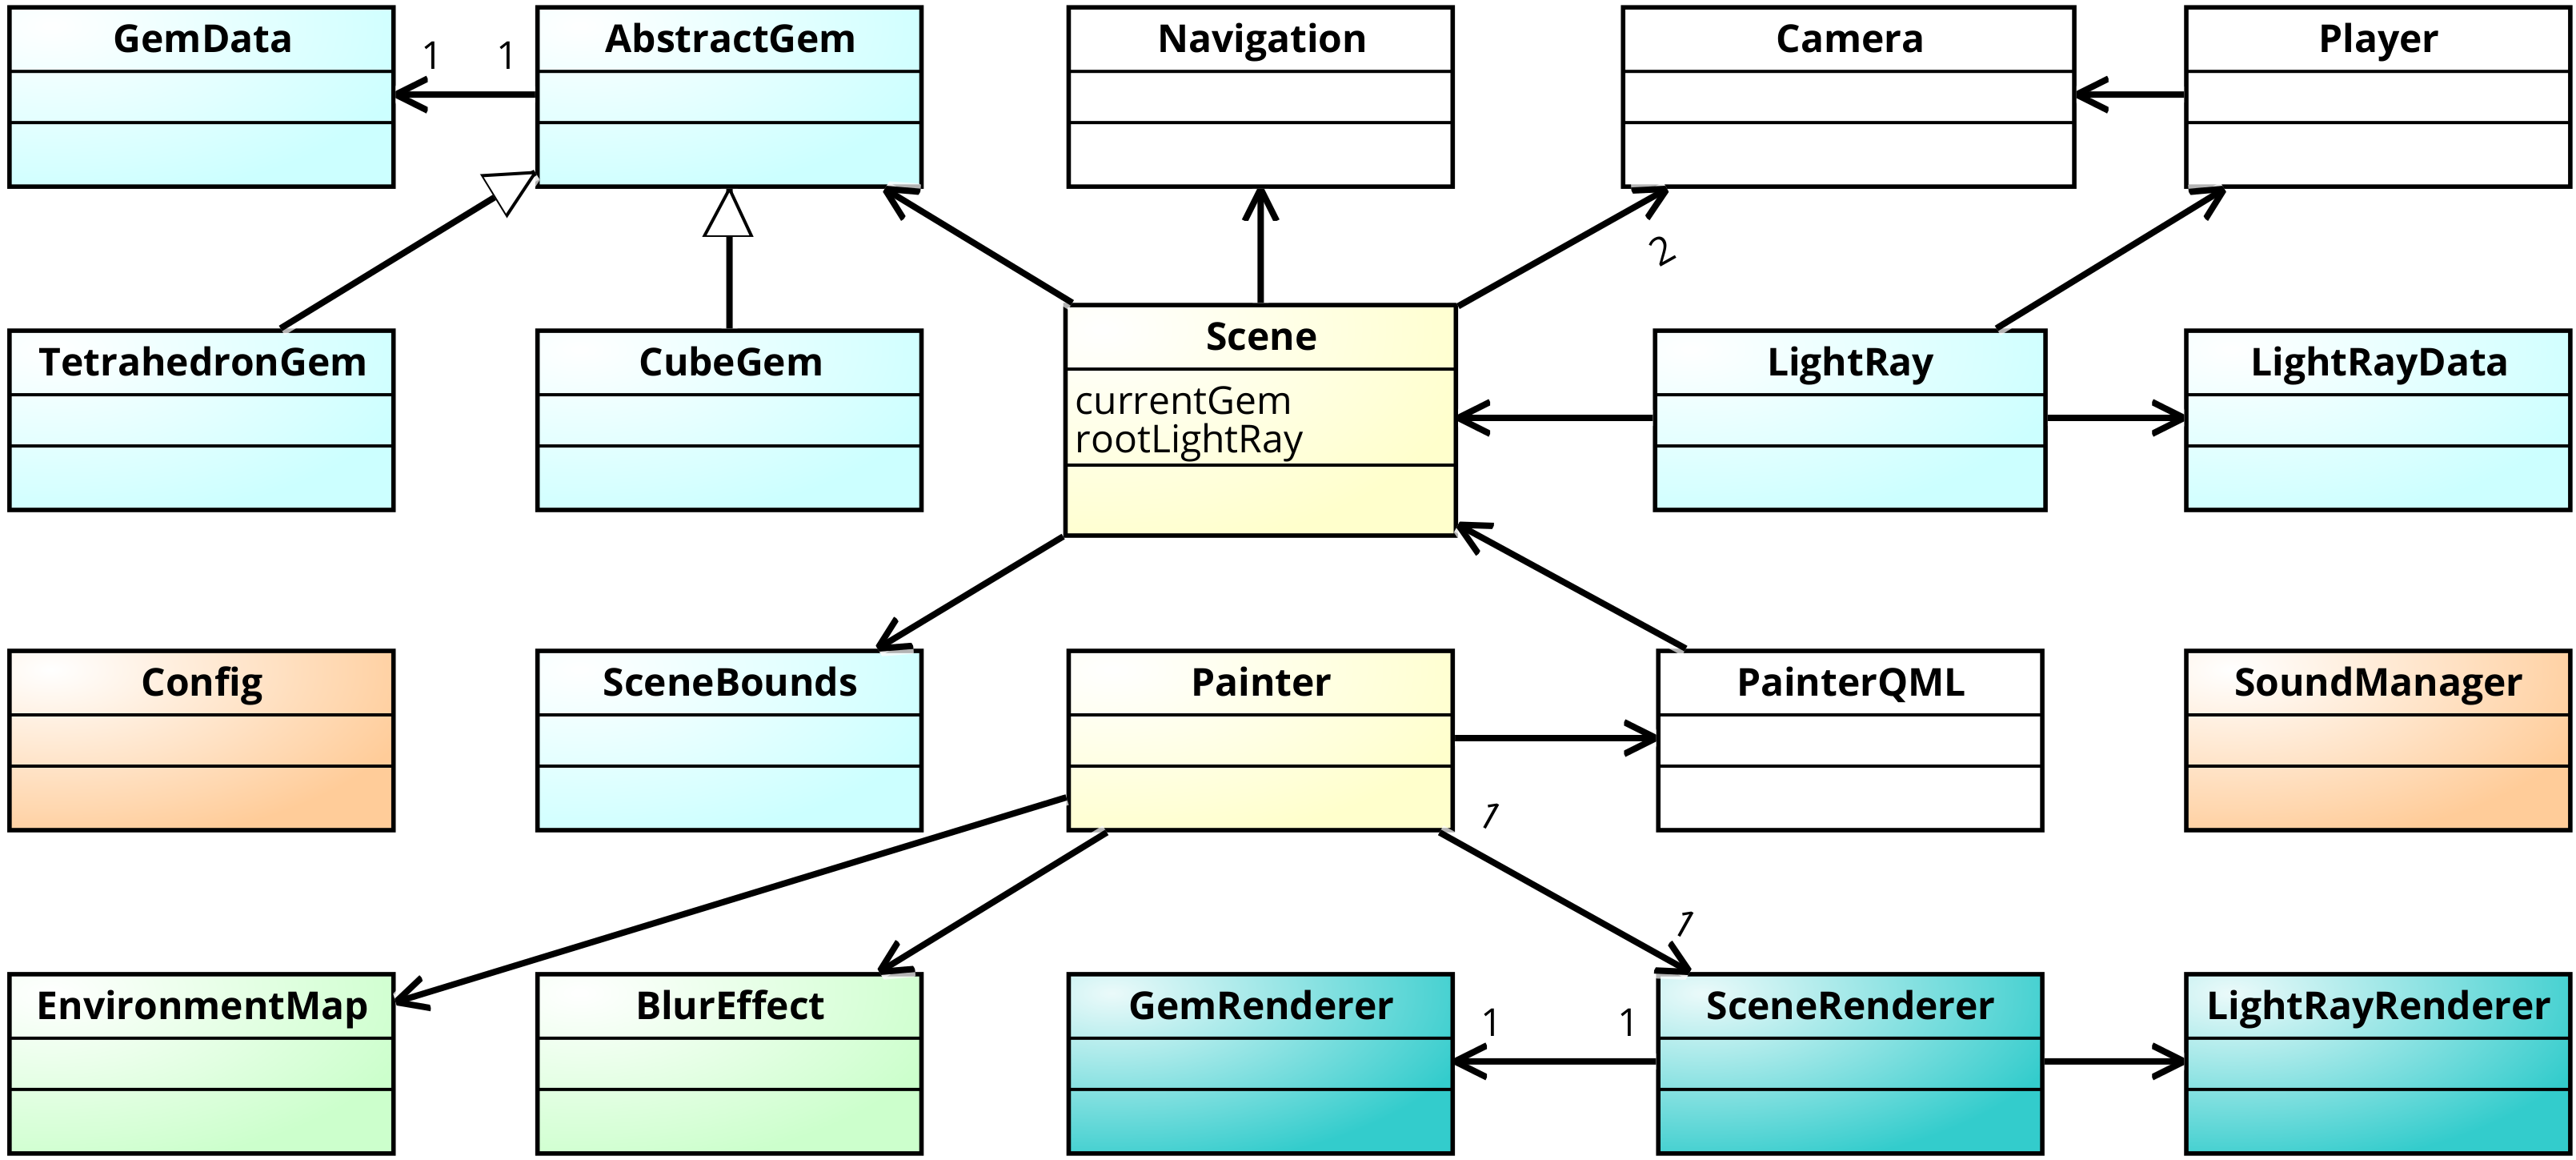
\includegraphics[width=\textwidth, height=0.7\textheight, keepaspectratio]{images/klassendiagramm-final}
	\end{figure}
\end{frame}

% 2m
\begin{frame}{Game Features}
	%Must-Haves, Should-Haves, Nice-To-Haves
	\begin{itemize}
		\item Start-Menü, Options-Menü mit Konfigurationsdatei, Ladebalken
		\item Kristalllandschaftgenerierung mit Seeds
		\item Verschiedene Kristalle
		\item Wechselnde Lichtstrahlfarbe
		\item Einfluss auf die Kristallfarbe
		\item Reflektion bei Kollision
		\item Pause-Button
		\item Hintergrundmusik und Soundeffekte
		\item Spielende und Highscore
	\end{itemize}
\end{frame}

% 2m
\begin{frame}{Computergraphic Features}
	\begin{itemize}
		\item Environment Mapping
		\item Reflektion und Refraktion der Environment Map in den Kristallen
		\item Preview Window 
		\item Glow-Effekt der Lichtstrahlen
	\end{itemize}
\end{frame}

% 1m
\begin{frame}{Technische Herausfordungen}
	\begin{itemize}
		\item Entwicklung auf 9 Geräten gleichzeitig
		\item Entwicklung für Grafikkarten von drei verschiedenen Herstellern 
		\item OpenGL ES 2.0
	\end{itemize}
\end{frame}

% 1m
\begin{frame}{Review: QML}
	\begin{itemize}
	\item QML Dokumentation
	\item QML Resource-Verwaltung und Assets
	\item QML: backgroundcolor: white vs. red
	\item Wage Fehlermeldungen
	\end{itemize}
\end{frame}

% 2m
\begin{frame}{Optimiertes Rendering}

\end{frame}

% 2m
\begin{frame}{Preview Window \& Glow}

\end{frame}

% 2m
\begin{frame}{Lessons learned}
	\begin{itemize}
		\item Abgleichen der Fähigkeiten, Erwartungen und Coding Styles
		\item Zufällig passendes Team
		\item Konstantes Arbeiten
		\item Spaß
	\end{itemize}
	\vfill
	\begin{itemize}
		\item Das Nachmittagstief
	\end{itemize}
\end{frame}

%\begin{frame}[allowframebreaks]{Bibliographie}
  \bibliographystyle{apalike}
  \bibliography{../../references}
  \vfill
\end{frame}

\end{document}
